% !TEX root = ../../ctfp-print.tex

\lettrine[lhang=0.17]{T}{he Ancient Greek} playwright Euripides once said: ``Every man is like
the company he is wont to keep.'' We are defined by our relationships.
Nowhere is this more true than in category theory. If we want to single
out a particular object in a category, we can only do this by describing
its pattern of relationships with other objects (and itself). These
relationships are defined by morphisms.

There is a common construction in category theory called the
\newterm{universal construction} for defining objects in terms of their
relationships. One way of doing this is to pick a pattern, a particular
shape constructed from objects and morphisms, and look for all its
occurrences in the category. If it's a common enough pattern, and the
category is large, chances are you'll have lots and lots of hits. The
trick is to establish some kind of ranking among those hits, and pick
what could be considered the best fit.

This process is reminiscent of the way we do web searches. A query is
like a pattern. A very general query will give you large \emph{recall}:
lots of hits. Some may be relevant, others not. To eliminate irrelevant
hits, you refine your query. That increases its \emph{precision}.
Finally, the search engine will rank the hits and, hopefully, the one
result that you're interested in will be at the top of the list.

\section{Initial Object}

The simplest shape is a single object. Obviously, there are as many
instances of this shape as there are objects in a given category. That's
a lot to choose from. We need to establish some kind of ranking and try
to find the object that tops this hierarchy. The only means at our
disposal are morphisms. If you think of morphisms as arrows, then it's
possible that there is an overall net flow of arrows from one end of the
category to another. This is true in ordered categories, for instance in
partial orders. We could generalize that notion of object precedence by
saying that object $a$ is ``more initial'' than object $b$, if
there is an arrow (a morphism) going from $a$ to $b$. We would
then define \emph{the} initial object as one that has arrows going to
all other objects. Obviously there is no guarantee that such an object
exists, and that's okay. A bigger problem is that there may be too many
such objects: The recall is good, but precision is lacking. The solution
is to take a hint from ordered categories --- they allow at most one
arrow between any two objects: there is only one way of being less-than
or equal-to another object. Which leads us to this definition of the
initial object:

\begin{quote}
The \textbf{initial object} is the object that has one and only one
morphism going to any object in the category.
\end{quote}

\begin{figure}[H]
\centering
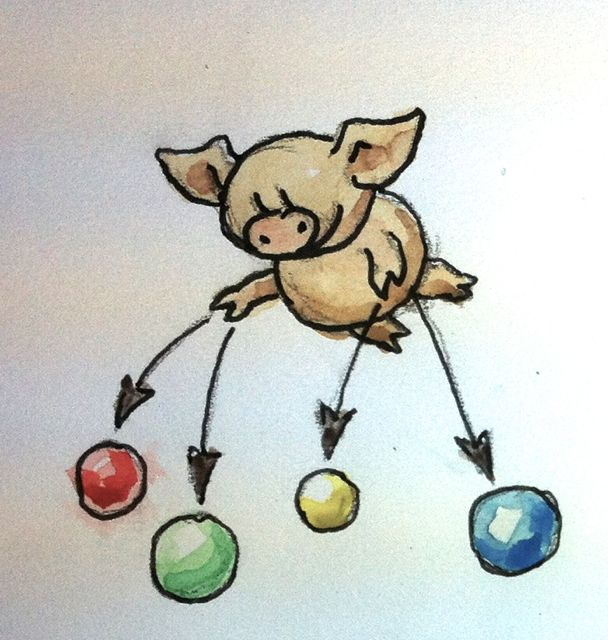
\includegraphics[width=40mm]{images/initial.jpg}
\end{figure}

\noindent
However, even that doesn't guarantee the uniqueness of the initial
object (if one exists). But it guarantees the next best thing:
uniqueness \newterm{up to isomorphism}. Isomorphisms are very important in
category theory, so I'll talk about them shortly. For now, let's just
agree that uniqueness up to isomorphism justifies the use of ``the'' in
the definition of the initial object.

Here are some examples: The initial object in a partially ordered set
(often called a \newterm{poset}) is its least element. Some posets don't
have an initial object --- like the set of all integers, positive and
negative, with less-than-or-equal relation for morphisms.

In the category of sets and functions, the initial object is the empty
set. Remember, an empty set corresponds to the Haskell type
\code{Void} (there is no corresponding type in C++) and the unique
polymorphic function from \code{Void} to any other type is called
\code{absurd}:

\src{snippet01}
It's this family of morphisms that makes \code{Void} the initial
object in the category of types.

\section{Terminal Object}

Let's continue with the single-object pattern, but let's change the way
we rank the objects. We'll say that object $a$ is ``more terminal''
than object $b$ if there is a morphism going from $b$ to
$a$ (notice the reversal of direction). We'll be looking for an
object that's more terminal than any other object in the category.
Again, we will insist on uniqueness:

\begin{quote}
The \textbf{terminal object} is the object with one and only one
morphism coming to it from any object in the category.
\end{quote}

\begin{figure}[H]
\centering
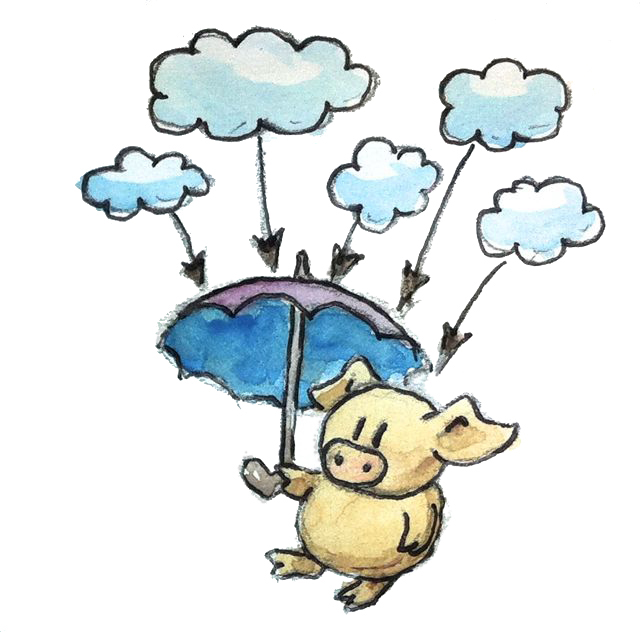
\includegraphics[width=40mm]{images/final.jpg}
\end{figure}

\noindent
And again, the terminal object is unique, up to isomorphism, which I
will show shortly. But first let's look at some examples. In a poset,
the terminal object, if it exists, is the biggest object. In the
category of sets, the terminal object is a singleton. We've already
talked about singletons --- they correspond to the \code{void} type in
C++ and the unit type \code{()} in Haskell. It's a type that has only
one value --- implicit in C++ and explicit in Haskell, denoted by
\code{()}. We've also established that there is one and only one pure
function from any type to the unit type:

\src{snippet02}
so all the conditions for the terminal object are satisfied.

Notice that in this example the uniqueness condition is crucial, because
there are other sets (actually, all of them, except for the empty set)
that have incoming morphisms from every set. For instance, there is a
Boolean-valued function (a predicate) defined for every type:

\src{snippet03}
But \code{Bool} is not a terminal object. There is at least one more
\code{Bool}-valued function from every type:

\src{snippet04}
Insisting on uniqueness gives us just the right precision to narrow down
the definition of the terminal object to just one type.

\section{Duality}

You can't help but to notice the symmetry between the way we defined the
initial object and the terminal object. The only difference between the
two was the direction of morphisms. It turns out that for any category $\cat{C}$
we can define the \newterm{opposite category} $\cat{C}^{op}$ just by
reversing all the arrows. The opposite category automatically satisfies
all the requirements of a category, as long as we simultaneously
redefine composition. If original morphisms
$f \Colon a \to b$ and $g \Colon b \to c$ composed
to $h \Colon a \to c$ with $h = g \circ f$, then the reversed
morphisms $f^{op} \Colon b \to a$ and $g^{op} \Colon c \to b$ will compose to
$h^{op} \Colon c \to a$ with $h^{op} = f^{op} \circ g^{op}$. And reversing
the identity arrows is a (pun alert!) no-op.

Duality is a very important property of categories because it doubles
the productivity of every mathematician working in category theory. For
every construction you come up with, there is its opposite; and for
every theorem you prove, you get one for free. The constructions in the
opposite category are often prefixed with ``co'', so you have products
and coproducts, monads and comonads, cones and cocones, limits and
colimits, and so on. There are no cocomonads though, because reversing
the arrows twice gets us back to the original state.

It follows then that a terminal object is the initial object in the
opposite category.

\section{Isomorphisms}

As programmers, we are well aware that defining equality is a nontrivial
task. What does it mean for two objects to be equal? Do they have to
occupy the same location in memory (pointer equality)? Or is it enough
that the values of all their components are equal? Are two complex
numbers equal if one is expressed as the real and imaginary part, and
the other as modulus and angle? You'd think that mathematicians would
have figured out the meaning of equality, but they haven't. They have
the same problem of multiple competing definitions for equality. There
is the propositional equality, intensional equality, extensional
equality, and equality as a path in homotopy type theory. And then there
are the weaker notions of isomorphism, and even weaker of equivalence.

The intuition is that isomorphic objects look the same --- they have the
same shape. It means that every part of one object corresponds to some
part of another object in a one-to-one mapping. As far as our
instruments can tell, the two objects are a perfect copy of each other.
Mathematically it means that there is a mapping from object $a$ to
object $b$, and there is a mapping from object $b$ back to
object $a$, and they are the inverse of each other. In category
theory we replace mappings with morphisms. An isomorphism is an
invertible morphism; or a pair of morphisms, one being the inverse of
the other.

We understand the inverse in terms of composition and identity: Morphism
$g$ is the inverse of morphism $f$ if their composition is the
identity morphism. These are actually two equations because there are
two ways of composing two morphisms:

\src{snippet05}
When I said that the initial (terminal) object was unique up to
isomorphism, I meant that any two initial (terminal) objects are
isomorphic. That's actually easy to see. Let's suppose that we have two
initial objects $i_{1}$ and $i_{2}$. Since
$i_{1}$ is initial, there is a unique morphism $f$ from
$i_{1}$ to $i_{2}$. By the same token, since
$i_{2}$ is initial, there is a unique morphism $g$ from
$i_{2}$ to $i_{1}$. What's the composition of
these two morphisms?

\begin{figure}[H]
\centering
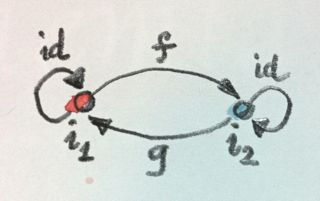
\includegraphics[width=40mm]{images/uniqueness.jpg}
\caption{All morphisms in this diagram are unique.}
\end{figure}

\noindent
The composition $g \circ f$ must be a morphism from $i_{1}$ to
$i_{1}$. But $i_{1}$ is initial so there can only
be one morphism going from $i_{1}$ to $i_{1}$.
Since we are in a category, we know that there is an identity morphism
from $i_{1}$ to $i_{1}$, and since there is room
for only one, that must be it. Therefore $g \circ f$ is equal to
identity. Similarly, $f \circ g$ must be equal to identity, because there
can be only one morphism from $i_{2}$ back to
$i_{2}$. This proves that $f$ and $g$ must be the
inverse of each other. Therefore any two initial objects are isomorphic.

Notice that in this proof we used the uniqueness of the morphism from
the initial object to itself. Without that we couldn't prove the ``up to
isomorphism'' part. But why do we need the uniqueness of $f$ and
$g$? Because not only is the initial object unique up to
isomorphism, it is unique up to \emph{unique} isomorphism. In principle,
there could be more than one isomorphism between two objects, but that's
not the case here. This ``uniqueness up to unique isomorphism'' is the
important property of all universal constructions.

\section{Products}

The next universal construction is that of a product. We know what a
Cartesian product of two sets is: it's a set of pairs. But what's the
pattern that connects the product set with its constituent sets? If we
can figure that out, we'll be able to generalize it to other categories.

All we can say is that there are two functions, the projections, from
the product to each of the constituents. In Haskell, these two functions
are called \code{fst} and \code{snd} and they pick, respectively,
the first and the second component of a pair:

\src{snippet06}

\src{snippet07}
Here, the functions are defined by pattern matching their arguments: the
pattern that matches any pair is \code{(x, y)}, and it extracts its
components into variables \code{x} and \code{y}.

These definitions can be simplified even further with the use of
wildcards:

\src{snippet08}
In C++, we would use template functions, for instance:

\begin{Verbatim}
template<class A, class B> A
fst(pair<A, B> const & p) {
    return p.first;
}
\end{Verbatim}
Equipped with this seemingly very limited knowledge, let's try to define
a pattern of objects and morphisms in the category of sets that will
lead us to the construction of a product of two sets, $a$ and
$b$. This pattern consists of an object $c$ and two morphisms
$p$ and $q$ connecting it to $a$ and $b$,
respectively:

\src{snippet09}

\begin{figure}[H]
\centering
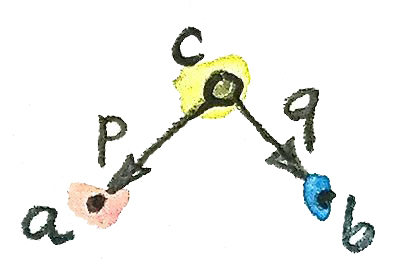
\includegraphics[width=40mm]{images/productpattern.jpg}
\end{figure}

\noindent
All $c$s that fit this pattern will be considered candidates for
the product. There may be lots of them.

\begin{figure}[H]
\centering
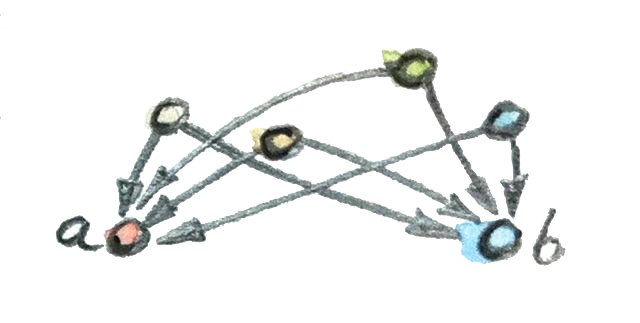
\includegraphics[width=40mm]{images/productcandidates.jpg}
\end{figure}

\noindent
For instance, let's pick, as our constituents, two Haskell types,
\code{Int} and \code{Bool}, and get a sampling of candidates for
their product.

Here's one: \code{Int}. Can \code{Int} be considered a candidate for
the product of \code{Int} and \code{Bool}? Yes, it can --- and here
are its projections:

\src{snippet10}
That's pretty lame, but it matches the criteria.

Here's another one: \code{(Int, Int, Bool)}. It's a tuple of three
elements, or a triple. Here are two morphisms that make it a legitimate
candidate (we are using pattern matching on triples):

\src{snippet11}
You may have noticed that while our first candidate was too small --- it
only covered the \code{Int} dimension of the product; the second was
too big --- it spuriously duplicated the \code{Int} dimension.

But we haven't explored yet the other part of the universal
construction: the ranking. We want to be able to compare two instances
of our pattern. We want to compare one candidate object $c$ and its
two projections $p$ and $q$ with another candidate object
$c'$ and its two projections $p'$ and $q'$. We would like
to say that $c$ is ``better'' than $c'$ if there is a morphism
$m$ from $c'$ to $c$ --- but that's too weak. We also
want its projections to be ``better,'' or ``more universal,'' than the
projections of $c'$. What it means is that the projections
$p'$ and $q'$ can be reconstructed from $p$ and $q$ using $m$:

\src{snippet12}

\begin{figure}[H]
\centering
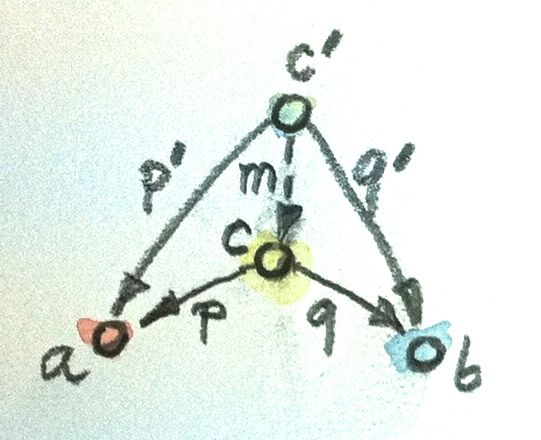
\includegraphics[width=40mm]{images/productranking.jpg}
\end{figure}

\noindent
Another way of looking at these equations is that $m$
\emph{factorizes} $p'$ and $q'$. Just pretend that these
equations are in natural numbers, and the dot is multiplication:
$m$ is a common factor shared by $p'$ and $q'$.

Just to build some intuitions, let me show you that the pair
\code{(Int, Bool)} with the two canonical projections, \code{fst}
and \code{snd} is indeed \emph{better} than the two candidates I
presented before.

\begin{figure}[H]
\centering
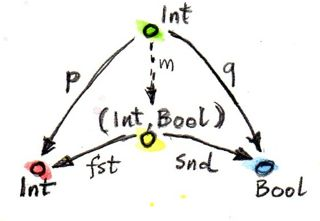
\includegraphics[width=50mm]{images/not-a-product.jpg}
\end{figure}

\noindent
The mapping \code{m} for the first candidate is:

\src{snippet13}
Indeed, the two projections, \code{p} and \code{q} can be
reconstructed as:

\src{snippet14}
The \code{m} for the second example is similarly uniquely determined:

\src{snippet15}
We were able to show that \code{(Int, Bool)} is better than either of
the two candidates. Let's see why the opposite is not true. Could we
find some \code{m'} that would help us reconstruct \code{fst}
and \code{snd} from \code{p} and \code{q}?

\src{snippet16}
In our first example, \code{q} always returned \code{True} and we
know that there are pairs whose second component is \code{False}. We
can't reconstruct \code{snd} from \code{q}.

The second example is different: we retain enough information after
running either \code{p} or \code{q}, but there is more than one way
to factorize \code{fst} and \code{snd}. Because both \code{p} and
\code{q} ignore the second component of the triple, our \code{m'}
can put anything in it. We can have:

\src{snippet17}

or
\src{snippet18}
and so on.

Putting it all together, given any type \code{c} with two projections
\code{p} and \code{q}, there is a unique \code{m} from \code{c}
to the Cartesian product \code{(a, b)} that factorizes them. In fact,
it just combines \code{p} and \code{q} into a pair.

\src{snippet19}
That makes the Cartesian product \code{(a, b)} our best match, which
means that this universal construction works in the category of sets. It
picks the product of any two sets.

Now let's forget about sets and define a product of two objects in any
category using the same universal construction. Such a product doesn't
always exist, but when it does, it is unique up to a unique isomorphism.

\begin{quote}
A \textbf{product} of two objects $a$ and $b$ is the object
$c$ equipped with two projections such that for any other object
$c'$ equipped with two projections there is a unique morphism
$m$ from $c'$ to $c$ that factorizes those projections.
\end{quote}

\noindent
A (higher order) function that produces the factorizing function
\code{m} from two candidates is sometimes called the
\newterm{factorizer}. In our case, it would be the function:

\src{snippet20}

\section{Coproduct}

Like every construction in category theory, the product has a dual,
which is called the coproduct. When we reverse the arrows in the product
pattern, we end up with an object $c$ equipped with two
\emph{injections}, \code{i} and \code{j}: morphisms from $a$
and $b$ to $c$.

\src{snippet21}

\begin{figure}[H]
\centering
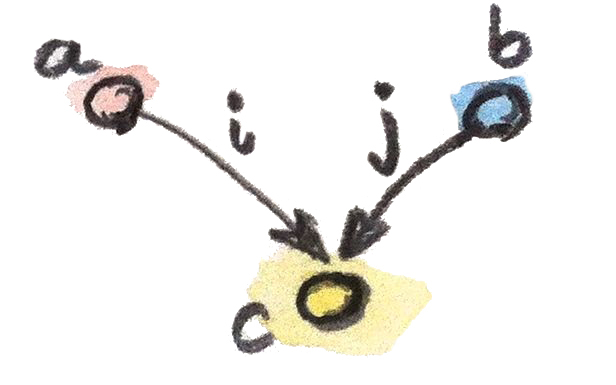
\includegraphics[width=40mm]{images/coproductpattern.jpg}
\end{figure}

\noindent
The ranking is also inverted: object $c$ is ``better'' than object
$c'$ that is equipped with the injections $i'$ and $j'$
if there is a morphism $m$ from $c$ to $c'$ that
factorizes the injections:

\src{snippet22}

\begin{figure}[H]
\centering
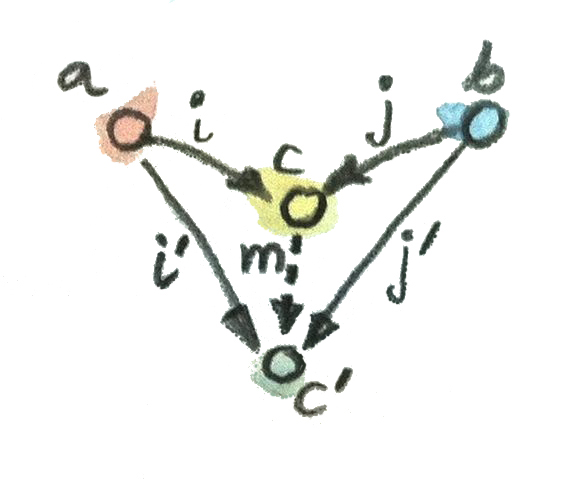
\includegraphics[width=40mm]{images/coproductranking.jpg}
\end{figure}

\noindent
The ``best'' such object, one with a unique morphism connecting it to
any other pattern, is called a coproduct and, if it exists, is unique up
to unique isomorphism.

\begin{quote}
A \textbf{coproduct} of two objects $a$ and $b$ is the object
$c$ equipped with two injections such that for any other object
$c'$ equipped with two injections there is a unique morphism
$m$ from $c$ to $c'$ that factorizes those injections.
\end{quote}

\noindent
In the category of sets, the coproduct is the \emph{disjoint union} of
two sets. An element of the disjoint union of $a$ and $b$ is
either an element of $a$ or an element of $b$. If the two sets
overlap, the disjoint union contains two copies of the common part. You
can think of an element of a disjoint union as being tagged with an
identifier that specifies its origin.

For a programmer, it's easier to understand a coproduct in terms of
types: it's a tagged union of two types. C++ supports unions, but they
are not tagged. It means that in your program you have to somehow keep
track which member of the union is valid. To create a tagged union, you
have to define a tag --- an enumeration --- and combine it with the
union. For instance, a tagged union of an \code{int} and a\\
\code{char const *} could be implemented as:

\begin{Verbatim}
struct Contact { 
    enum { isPhone, isEmail } tag;
    union { int phoneNum; char const * emailAddr; };
};
\end{Verbatim}
The two injections can either be implemented as constructors or as
functions. For instance, here's the first injection as a function
\code{PhoneNum}:

\begin{Verbatim}
Contact PhoneNum(int n) { 
    Contact c;
    c.tag = isPhone;
    c.phoneNum = n;
    return c;
}
\end{Verbatim}
It injects an integer into \code{Contact}.

A tagged union is also called a \newterm{variant}, and there is a very
general implementation of a variant in the boost library,
\code{boost::variant}.

In Haskell, you can combine any data types into a tagged union by
separating data constructors with a vertical bar. The \code{Contact}
example translates into the declaration:

\src{snippet23}
Here, \code{PhoneNum} and \code{EmailAddr} serve both as
constructors (injections), and as tags for pattern matching (more about
this later). For instance, this is how you would construct a contact
using a phone number:

\src{snippet24}
Unlike the canonical implementation of the product that is built into
Haskell as the primitive pair, the canonical implementation of the
coproduct is a data type called \code{Either}, which is defined in the
standard Prelude as:

\src{snippet25}
It is parameterized by two types, \code{a} and \code{b} and has two
constructors: \code{Left} that takes a value of type \code{a}, and
\code{Right} that takes a value of type \code{b}.

Just as we've defined the factorizer for a product, we can define one
for the coproduct. Given a candidate type \code{c} and two candidate
injections \code{i} and \code{j}, the factorizer for \code{Either}
produces the factoring function:

\src{snippet26}

\section{Asymmetry}

We've seen two sets of dual definitions: The definition of a terminal
object can be obtained from the definition of the initial object by
reversing the direction of arrows; in a similar way, the definition of
the coproduct can be obtained from that of the product. Yet in the
category of sets the initial object is very different from the final
object, and coproduct is very different from product. We'll see later
that product behaves like multiplication, with the terminal object
playing the role of one; whereas coproduct behaves more like the sum,
with the initial object playing the role of zero. In particular, for
finite sets, the size of the product is the product of the sizes of
individual sets, and the size of the coproduct is the sum of the sizes.

This shows that the category of sets is not symmetric with respect to
the inversion of arrows.

Notice that while the empty set has a unique morphism to any set (the
\code{absurd} function), it has no morphisms coming back. The
singleton set has a unique morphism coming to it from any set, but it
\emph{also} has outgoing morphisms to every set (except for the empty
one). As we've seen before, these outgoing morphisms from the terminal
object play a very important role of picking elements of other sets (the
empty set has no elements, so there's nothing to pick).

It's the relationship of the singleton set to the product that sets it
apart from the coproduct. Consider using the singleton set, represented
by the unit type \code{()}, as yet another --- vastly inferior ---
candidate for the product pattern. Equip it with two projections
\code{p} and \code{q}: functions from the singleton to each of the
constituent sets. Each selects a concrete element from either set.
Because the product is universal, there is also a (unique) morphism
\code{m} from our candidate, the singleton, to the product. This
morphism selects an element from the product set --- it selects a
concrete pair. It also factorizes the two projections:

\src{snippet27}
When acting on the singleton value \code{()}, the only element of the
singleton set, these two equations become:

\src{snippet28}
Since \code{m ()} is the element of the product picked by \code{m},
these equations tell us that the element picked by \code{p} from the
first set, \code{p ()}, is the first component of the pair picked by
\code{m}. Similarly, \code{q ()} is equal to the second component.
This is in total agreement with our understanding that elements of the
product are pairs of elements from the constituent sets.

There is no such simple interpretation of the coproduct. We could try
the singleton set as a candidate for a coproduct, in an attempt to
extract the elements from it, but there we would have two injections
going into it rather than two projections coming out of it. They'd tell
us nothing about their sources (in fact, we've seen that they ignore the
input parameter). Neither would the unique morphism from the coproduct
to our singleton. The category of sets just looks very different when
seen from the direction of the initial object than it does when seen
from the terminal end.

This is not an intrinsic property of sets, it's a property of functions,
which we use as morphisms in $\Set$. Functions are, in general,
asymmetric. Let me explain.

A function must be defined for every element of its domain set (in
programming, we call it a \newterm{total} function), but it doesn't have to
cover the whole codomain. We've seen some extreme cases of it: functions
from a singleton set --- functions that select just a single element in
the codomain. (Actually, functions from an empty set are the real
extremes.) When the size of the domain is much smaller than the size of
the codomain, we often think of such functions as embedding the domain
in the codomain. For instance, we can think of a function from a
singleton set as embedding its single element in the codomain. I call
them \newterm{embedding} functions, but mathematicians prefer to give a
name to the opposite: functions that tightly fill their codomains are
called \newterm{surjective} or \newterm{onto}.

The other source of asymmetry is that functions are allowed to map many
elements of the domain set into one element of the codomain. They can
collapse them. The extreme case are functions that map whole sets into a
singleton. You've seen the polymorphic \code{unit} function that does
just that. The collapsing can only be compounded by composition. A
composition of two collapsing functions is even more collapsing than the
individual functions. Mathematicians have a name for non-collapsing
functions: they call them \newterm{injective} or \newterm{one-to-one}.

Of course there are some functions that are neither embedding nor
collapsing. They are called \newterm{bijections} and they are truly
symmetric, because they are invertible. In the category of sets, an
isomorphism is the same as a bijection.

\section{Challenges}

\begin{enumerate}
\tightlist
\item
  Show that the terminal object is unique up to unique isomorphism.
\item
  What is a product of two objects in a poset? Hint: Use the universal
  construction.
\item
  What is a coproduct of two objects in a poset?
\item
  Implement the equivalent of Haskell \code{Either} as a generic type
  in your favorite language (other than Haskell).
\item
  Show that \code{Either} is a ``better'' coproduct than \code{int}
  equipped with two injections:

\begin{Verbatim}
int i(int n) { return n; }
int j(bool b) { return b ? 0: 1; }
\end{Verbatim}

  Hint: Define a function

\begin{Verbatim}
int m(Either const & e);
\end{Verbatim}

  that factorizes \code{i} and \code{j}.
\item
  Continuing the previous problem: How would you argue that \code{int}
  with the two injections \code{i} and \code{j} cannot be ``better''
  than \code{Either}?
\item
  Still continuing: What about these injections?

\begin{Verbatim}
int i(int n) { 
    if (n < 0) return n;
    return n + 2;
}

int j(bool b) { return b ? 0: 1; }
\end{Verbatim}
\item
  Come up with an inferior candidate for a coproduct of \code{int} and
  \code{bool} that cannot be better than \code{Either} because it
  allows multiple acceptable morphisms from it to \code{Either}.
\end{enumerate}

\section{Bibliography}

\begin{enumerate}
\tightlist
\item
  The Catsters,
  \urlref{https://www.youtube.com/watch?v=upCSDIO9pjc}{Products and
  Coproducts} video.
\end{enumerate}
